\documentclass{article}
\usepackage{graphicx}
\begin{document}
\hfill Alejandro Chavez

\hfill Assignment 4 - Digital Logic

\hfill \today\\

\begin{center}\begin{large}Assignment 4\end{large}\end{center}	Chapter 4 Exercises
\begin{itemize}
	\item
		1)\\
		$0110_{10} + 0011_{10} = 1001_{10}$\\
		$6+3 =9$
	\item
		2)\\
		$1110 + 0111 = (1)0101$\\
		$-2 + 7 = 5$\\
		This addition does not result in an overflow because $1110$ and $0111$ do not share the same sign. 
	\item
		3)\\
    Partly. The result on an overflowing output bus is the negation of the correct answer. When overflow occurs, the processor should send the result in a bigger memory space and put the correct sign bit in the right place.
  \item
    4)\\
    $0xBA+0x7F=0x(1)39$\\
    $10111010+01111111=(1)00111001$\\
    $-70+127=57$\\
    This addition also does not result in an overflow because the signs are not the same on either operand.
  \item
    5)\\
    $1110 +1001 = 10111$\\
    $-2 + -7 = -9$\\
    This addition does result in overflow. The sign bit gets pushed to the next largest bit (the 5th bit).
  \item
    6)\\
    \begin{tabular}{ccc|c}
    $A$ & $B$ & $Cin$ & $Sum$ \\ \hline
    $x$ & $y$ & $Cin$ & if $-128<x+y+Cin<127$ , $x+y$ ; else $(x+y+Cin)-256$\\
    \end{tabular}
  \item
    7)\\
    If $Sa+Sb+Cout$ then $Ovfl$\\
    Other than that, Overflow may or may not happen with the given signals.
  \item
    8)\\
    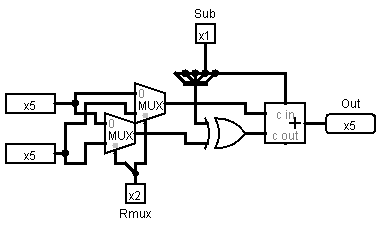
\includegraphics[scale=0.5]{ass4-8.png}
  \item
    10)\\
    The $Inv.$ block is just one XOR gate.\\
    The $Neg.$ block may consist of a NOT gate on each bit and minus one the number of bits of the signal one bit full adders. The one bit full adder I built consisted of 8 gates, so for an 8 bit signal, a $Neg.$ block may consist of 8+8*7 = 64 gates. Ill take the $Inv.$ block, thank you.
  \item
    11)\\
    Because to fully negate signal $B$, it must add 1 to it, otherwise it would just be inverting it.
    \item
    12)\\
    The borrow signal returns 1 when B is trying to subtract from a number greater than itself if B is negative.\\
    I actually don't know. I don't think this is right. I will ask this in class.
\end{itemize}
\end{document}
